\documentclass[]{book}
\usepackage{lmodern}
\usepackage{amssymb,amsmath}
\usepackage{ifxetex,ifluatex}
\usepackage{fixltx2e} % provides \textsubscript
\ifnum 0\ifxetex 1\fi\ifluatex 1\fi=0 % if pdftex
  \usepackage[T1]{fontenc}
  \usepackage[utf8]{inputenc}
\else % if luatex or xelatex
  \ifxetex
    \usepackage{mathspec}
  \else
    \usepackage{fontspec}
  \fi
  \defaultfontfeatures{Ligatures=TeX,Scale=MatchLowercase}
\fi
% use upquote if available, for straight quotes in verbatim environments
\IfFileExists{upquote.sty}{\usepackage{upquote}}{}
% use microtype if available
\IfFileExists{microtype.sty}{%
\usepackage{microtype}
\UseMicrotypeSet[protrusion]{basicmath} % disable protrusion for tt fonts
}{}
\usepackage[margin=1in]{geometry}
\usepackage{hyperref}
\hypersetup{unicode=true,
            pdftitle={Data Science With Python},
            pdfauthor={L A Liggett},
            pdfborder={0 0 0},
            breaklinks=true}
\urlstyle{same}  % don't use monospace font for urls
\usepackage{natbib}
\bibliographystyle{apalike}
\usepackage{color}
\usepackage{fancyvrb}
\newcommand{\VerbBar}{|}
\newcommand{\VERB}{\Verb[commandchars=\\\{\}]}
\DefineVerbatimEnvironment{Highlighting}{Verbatim}{commandchars=\\\{\}}
% Add ',fontsize=\small' for more characters per line
\usepackage{framed}
\definecolor{shadecolor}{RGB}{248,248,248}
\newenvironment{Shaded}{\begin{snugshade}}{\end{snugshade}}
\newcommand{\KeywordTok}[1]{\textcolor[rgb]{0.13,0.29,0.53}{\textbf{#1}}}
\newcommand{\DataTypeTok}[1]{\textcolor[rgb]{0.13,0.29,0.53}{#1}}
\newcommand{\DecValTok}[1]{\textcolor[rgb]{0.00,0.00,0.81}{#1}}
\newcommand{\BaseNTok}[1]{\textcolor[rgb]{0.00,0.00,0.81}{#1}}
\newcommand{\FloatTok}[1]{\textcolor[rgb]{0.00,0.00,0.81}{#1}}
\newcommand{\ConstantTok}[1]{\textcolor[rgb]{0.00,0.00,0.00}{#1}}
\newcommand{\CharTok}[1]{\textcolor[rgb]{0.31,0.60,0.02}{#1}}
\newcommand{\SpecialCharTok}[1]{\textcolor[rgb]{0.00,0.00,0.00}{#1}}
\newcommand{\StringTok}[1]{\textcolor[rgb]{0.31,0.60,0.02}{#1}}
\newcommand{\VerbatimStringTok}[1]{\textcolor[rgb]{0.31,0.60,0.02}{#1}}
\newcommand{\SpecialStringTok}[1]{\textcolor[rgb]{0.31,0.60,0.02}{#1}}
\newcommand{\ImportTok}[1]{#1}
\newcommand{\CommentTok}[1]{\textcolor[rgb]{0.56,0.35,0.01}{\textit{#1}}}
\newcommand{\DocumentationTok}[1]{\textcolor[rgb]{0.56,0.35,0.01}{\textbf{\textit{#1}}}}
\newcommand{\AnnotationTok}[1]{\textcolor[rgb]{0.56,0.35,0.01}{\textbf{\textit{#1}}}}
\newcommand{\CommentVarTok}[1]{\textcolor[rgb]{0.56,0.35,0.01}{\textbf{\textit{#1}}}}
\newcommand{\OtherTok}[1]{\textcolor[rgb]{0.56,0.35,0.01}{#1}}
\newcommand{\FunctionTok}[1]{\textcolor[rgb]{0.00,0.00,0.00}{#1}}
\newcommand{\VariableTok}[1]{\textcolor[rgb]{0.00,0.00,0.00}{#1}}
\newcommand{\ControlFlowTok}[1]{\textcolor[rgb]{0.13,0.29,0.53}{\textbf{#1}}}
\newcommand{\OperatorTok}[1]{\textcolor[rgb]{0.81,0.36,0.00}{\textbf{#1}}}
\newcommand{\BuiltInTok}[1]{#1}
\newcommand{\ExtensionTok}[1]{#1}
\newcommand{\PreprocessorTok}[1]{\textcolor[rgb]{0.56,0.35,0.01}{\textit{#1}}}
\newcommand{\AttributeTok}[1]{\textcolor[rgb]{0.77,0.63,0.00}{#1}}
\newcommand{\RegionMarkerTok}[1]{#1}
\newcommand{\InformationTok}[1]{\textcolor[rgb]{0.56,0.35,0.01}{\textbf{\textit{#1}}}}
\newcommand{\WarningTok}[1]{\textcolor[rgb]{0.56,0.35,0.01}{\textbf{\textit{#1}}}}
\newcommand{\AlertTok}[1]{\textcolor[rgb]{0.94,0.16,0.16}{#1}}
\newcommand{\ErrorTok}[1]{\textcolor[rgb]{0.64,0.00,0.00}{\textbf{#1}}}
\newcommand{\NormalTok}[1]{#1}
\usepackage{longtable,booktabs}
\usepackage{graphicx,grffile}
\makeatletter
\def\maxwidth{\ifdim\Gin@nat@width>\linewidth\linewidth\else\Gin@nat@width\fi}
\def\maxheight{\ifdim\Gin@nat@height>\textheight\textheight\else\Gin@nat@height\fi}
\makeatother
% Scale images if necessary, so that they will not overflow the page
% margins by default, and it is still possible to overwrite the defaults
% using explicit options in \includegraphics[width, height, ...]{}
\setkeys{Gin}{width=\maxwidth,height=\maxheight,keepaspectratio}
\IfFileExists{parskip.sty}{%
\usepackage{parskip}
}{% else
\setlength{\parindent}{0pt}
\setlength{\parskip}{6pt plus 2pt minus 1pt}
}
\setlength{\emergencystretch}{3em}  % prevent overfull lines
\providecommand{\tightlist}{%
  \setlength{\itemsep}{0pt}\setlength{\parskip}{0pt}}
\setcounter{secnumdepth}{5}
% Redefines (sub)paragraphs to behave more like sections
\ifx\paragraph\undefined\else
\let\oldparagraph\paragraph
\renewcommand{\paragraph}[1]{\oldparagraph{#1}\mbox{}}
\fi
\ifx\subparagraph\undefined\else
\let\oldsubparagraph\subparagraph
\renewcommand{\subparagraph}[1]{\oldsubparagraph{#1}\mbox{}}
\fi

%%% Use protect on footnotes to avoid problems with footnotes in titles
\let\rmarkdownfootnote\footnote%
\def\footnote{\protect\rmarkdownfootnote}

%%% Change title format to be more compact
\usepackage{titling}

% Create subtitle command for use in maketitle
\newcommand{\subtitle}[1]{
  \posttitle{
    \begin{center}\large#1\end{center}
    }
}

\setlength{\droptitle}{-2em}

  \title{Data Science With Python}
    \pretitle{\vspace{\droptitle}\centering\huge}
  \posttitle{\par}
    \author{L A Liggett}
    \preauthor{\centering\large\emph}
  \postauthor{\par}
      \predate{\centering\large\emph}
  \postdate{\par}
    \date{2019-06-06}

\usepackage{booktabs}
\usepackage{amsthm}
\makeatletter
\def\thm@space@setup{%
  \thm@preskip=8pt plus 2pt minus 4pt
  \thm@postskip=\thm@preskip
}
\makeatother

\begin{document}
\maketitle

{
\setcounter{tocdepth}{1}
\tableofcontents
}
\chapter{Prerequisites}\label{prerequisites}

This is a \emph{sample} book written in \textbf{Markdown}. You can use
anything that Pandoc's Markdown supports, e.g., a math equation
\(a^2 + b^2 = c^2\).

The \textbf{bookdown} package can be installed from CRAN or Github:

\begin{Shaded}
\begin{Highlighting}[]
\KeywordTok{install.packages}\NormalTok{(}\StringTok{"bookdown"}\NormalTok{)}
\CommentTok{# or the development version}
\CommentTok{# devtools::install_github("rstudio/bookdown")}
\end{Highlighting}
\end{Shaded}

Remember each Rmd file contains one and only one chapter, and a chapter
is defined by the first-level heading \texttt{\#}.

To compile this example to PDF, you need XeLaTeX. You are recommended to
install TinyTeX (which includes XeLaTeX):
\url{https://yihui.name/tinytex/}.

\chapter{Introduction}\label{intro}

You can label chapter and section titles using \texttt{\{\#label\}}
after them, e.g., we can reference Chapter \ref{intro}. If you do not
manually label them, there will be automatic labels anyway, e.g.,
Chapter \ref{visualization}.

Figures and tables with captions will be placed in \texttt{figure} and
\texttt{table} environments, respectively.

And this is some other random stuff.

\begin{Shaded}
\begin{Highlighting}[]
\KeywordTok{par}\NormalTok{(}\DataTypeTok{mar =} \KeywordTok{c}\NormalTok{(}\DecValTok{4}\NormalTok{, }\DecValTok{4}\NormalTok{, .}\DecValTok{1}\NormalTok{, .}\DecValTok{1}\NormalTok{))}
\KeywordTok{plot}\NormalTok{(pressure, }\DataTypeTok{type =} \StringTok{'b'}\NormalTok{, }\DataTypeTok{pch =} \DecValTok{19}\NormalTok{)}
\end{Highlighting}
\end{Shaded}

\begin{figure}

{\centering 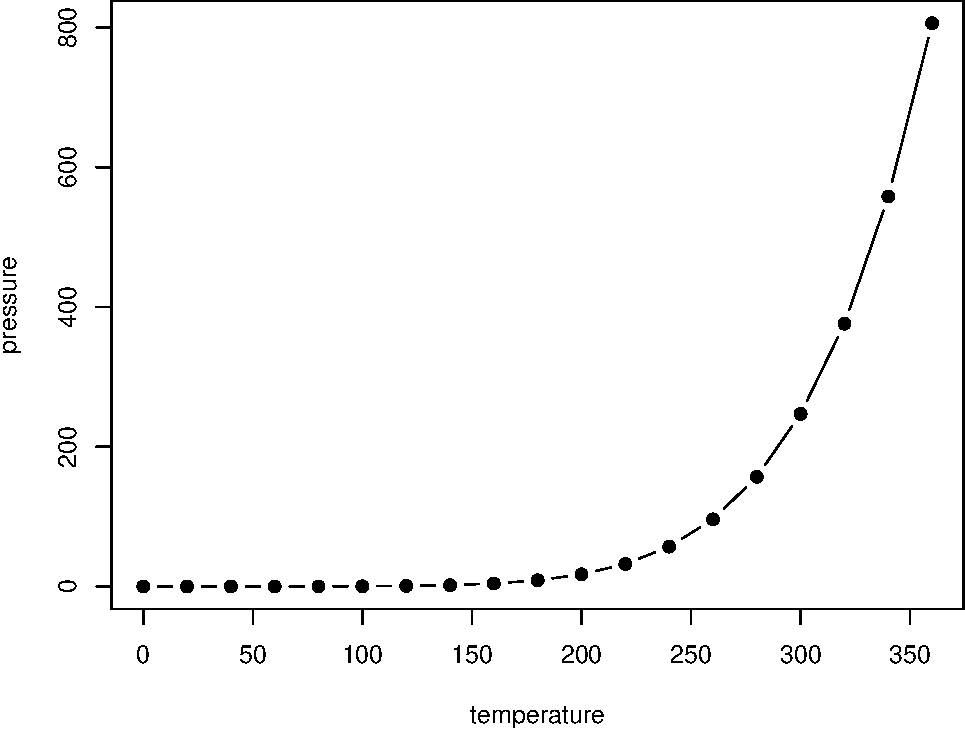
\includegraphics[width=0.8\linewidth]{bookdown-demo_files/figure-latex/nice-fig-1} 

}

\caption{Here is a nice figure!}\label{fig:nice-fig}
\end{figure}

Reference a figure by its code chunk label with the \texttt{fig:}
prefix, e.g., see Figure \ref{fig:nice-fig}. Similarly, you can
reference tables generated from \texttt{knitr::kable()}, e.g., see Table
\ref{tab:nice-tab}.

\begin{Shaded}
\begin{Highlighting}[]
\NormalTok{knitr}\OperatorTok{::}\KeywordTok{kable}\NormalTok{(}
  \KeywordTok{head}\NormalTok{(iris, }\DecValTok{20}\NormalTok{), }\DataTypeTok{caption =} \StringTok{'Here is a nice table!'}\NormalTok{,}
  \DataTypeTok{booktabs =} \OtherTok{TRUE}
\NormalTok{)}
\end{Highlighting}
\end{Shaded}

\begin{table}[t]

\caption{\label{tab:nice-tab}Here is a nice table!}
\centering
\begin{tabular}{rrrrl}
\toprule
Sepal.Length & Sepal.Width & Petal.Length & Petal.Width & Species\\
\midrule
5.1 & 3.5 & 1.4 & 0.2 & setosa\\
4.9 & 3.0 & 1.4 & 0.2 & setosa\\
4.7 & 3.2 & 1.3 & 0.2 & setosa\\
4.6 & 3.1 & 1.5 & 0.2 & setosa\\
5.0 & 3.6 & 1.4 & 0.2 & setosa\\
\addlinespace
5.4 & 3.9 & 1.7 & 0.4 & setosa\\
4.6 & 3.4 & 1.4 & 0.3 & setosa\\
5.0 & 3.4 & 1.5 & 0.2 & setosa\\
4.4 & 2.9 & 1.4 & 0.2 & setosa\\
4.9 & 3.1 & 1.5 & 0.1 & setosa\\
\addlinespace
5.4 & 3.7 & 1.5 & 0.2 & setosa\\
4.8 & 3.4 & 1.6 & 0.2 & setosa\\
4.8 & 3.0 & 1.4 & 0.1 & setosa\\
4.3 & 3.0 & 1.1 & 0.1 & setosa\\
5.8 & 4.0 & 1.2 & 0.2 & setosa\\
\addlinespace
5.7 & 4.4 & 1.5 & 0.4 & setosa\\
5.4 & 3.9 & 1.3 & 0.4 & setosa\\
5.1 & 3.5 & 1.4 & 0.3 & setosa\\
5.7 & 3.8 & 1.7 & 0.3 & setosa\\
5.1 & 3.8 & 1.5 & 0.3 & setosa\\
\bottomrule
\end{tabular}
\end{table}

\begin{Shaded}
\begin{Highlighting}[]
\NormalTok{knitr}\OperatorTok{::}\KeywordTok{include_graphics}\NormalTok{(}\KeywordTok{rep}\NormalTok{(}\StringTok{"knit-logo.png"}\NormalTok{, }\DecValTok{3}\NormalTok{))}
\end{Highlighting}
\end{Shaded}

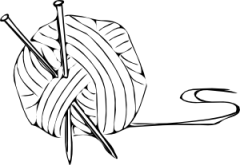
\includegraphics{knit-logo.png} 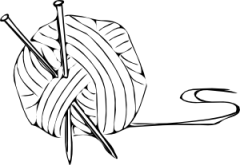
\includegraphics{knit-logo.png}
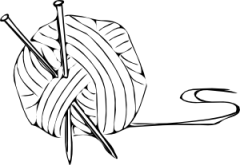
\includegraphics{knit-logo.png}

\begin{Shaded}
\begin{Highlighting}[]
\NormalTok{knitr}\OperatorTok{::}\KeywordTok{include_app}\NormalTok{(}\StringTok{"https://yihui.shinyapps.io/miniUI/"}\NormalTok{, }
                     \DataTypeTok{height =} \StringTok{"600px"}\NormalTok{)}
\end{Highlighting}
\end{Shaded}

\begin{Shaded}
\begin{Highlighting}[]
\ImportTok{import}\NormalTok{ pandas }\ImportTok{as}\NormalTok{ pd}
\NormalTok{x }\OperatorTok{=} \StringTok{'hello, python world!'}
\BuiltInTok{print}\NormalTok{(x.split(}\StringTok{' '}\NormalTok{))}
\end{Highlighting}
\end{Shaded}

\begin{verbatim}
## ['hello,', 'python', 'world!']
\end{verbatim}

You can write citations, too. For example, we are using the
\textbf{bookdown} package \citep{R-bookdown} in this sample book, which
was built on top of R Markdown and \textbf{knitr} \citep{xie2015}.

\chapter{JupyterLab}\label{jupyter}

Here is a simple template that I use that controls a couple useful
things when starting a new notebook.

\begin{Shaded}
\begin{Highlighting}[]
\ImportTok{import}\NormalTok{ sys}
\NormalTok{sys.path.append(}\StringTok{'../util'}\NormalTok{)}

\OperatorTok\NormalTok{autoreload }\DecValTok{2}

\ImportTok{from}\NormalTok{ util }\ImportTok{import} \OperatorTok{*}
\ImportTok{import}\NormalTok{ numpy }\ImportTok{as}\NormalTok{ np                  }
\ImportTok{import}\NormalTok{ pandas }\ImportTok{as}\NormalTok{ pd                 }
\ImportTok{from}\NormalTok{ matplotlib }\ImportTok{import}\NormalTok{ pyplot }\ImportTok{as}\NormalTok{ plt}
\ImportTok{import}\NormalTok{ seaborn }\ImportTok{as}\NormalTok{ sns}

\NormalTok{sns.set_palette(}\StringTok{'pastel'}\NormalTok{)}
\NormalTok{sns.set_style(}\StringTok{'ticks'}\NormalTok{)}
\NormalTok{sns.set_context(}\StringTok{'paper'}\NormalTok{, font_scale}\OperatorTok{=}\DecValTok{1}\NormalTok{)}
\end{Highlighting}
\end{Shaded}

It is often convenient to have a notebook automatically refresh the
imported libraries so that they can be modified while working on a
JupyterLab notebook.

\begin{Shaded}
\begin{Highlighting}[]
\OperatorTok\NormalTok{autoreload }\DecValTok{2}
\end{Highlighting}
\end{Shaded}

To allow directory organization, dependcies can be separated into
different directories and imported into a jupyter notebook using the
following import statement.

\begin{Shaded}
\begin{Highlighting}[]
\ImportTok{import}\NormalTok{ sys}
\NormalTok{sys.path.append(}\StringTok{'../util'}\NormalTok{)}
\end{Highlighting}
\end{Shaded}

A table of contents can be created to refer to each of the headers
throughout a notebook in html format. The code is below (Obviously needs
to be simplified.)

\begin{Shaded}
\begin{Highlighting}[]
\KeywordTok{<h1>}\NormalTok{Table of Contents}\KeywordTok{<span}\OtherTok{ class=}\StringTok{"tocSkip"}\KeywordTok{></span></h1>}
\KeywordTok{<div}\OtherTok{ class=}\StringTok{"toc"}\KeywordTok{>}
    \KeywordTok{<ul}\OtherTok{ class=}\StringTok{"toc-item"}\KeywordTok{>}
    \KeywordTok{<li>}
        \KeywordTok{<span><a}\OtherTok{ href=}\StringTok{"#Python-Setup"}\OtherTok{ data-toc-modified-id=}\StringTok{"Python-Setup-1"}\KeywordTok{><span}\OtherTok{ class=}\StringTok{"toc-item-num"}\KeywordTok{>}\NormalTok{1}\DecValTok{&nbsp;&nbsp;}\KeywordTok{</span>}\NormalTok{Python Setup}\KeywordTok{</a></span>}
        \KeywordTok{<ul}\OtherTok{ class=}\StringTok{"toc-item"}\KeywordTok{>}
    \KeywordTok{<li>}
        \KeywordTok{<span><a}\OtherTok{ href=}\StringTok{"#Change-the-width-of-the-page"}\OtherTok{ data-toc-modified-id=}\StringTok{"Change-the-width-of-the-page-1.1"}\KeywordTok{><span}\OtherTok{ class=}\StringTok{"toc-item-num"}\KeywordTok{>}\NormalTok{1.1}\DecValTok{&nbsp;&nbsp;}\KeywordTok{</span>}\NormalTok{Change the width of the page}\KeywordTok{</a></span></li>}
        \KeywordTok{<li>}
            \KeywordTok{<span><a}\OtherTok{ href=}\StringTok{"#Import-packages"}\OtherTok{ data-toc-modified-id=}\StringTok{"Import-packages-1.2"}\KeywordTok{><span}\OtherTok{ class=}\StringTok{"toc-item-num"}\KeywordTok{>}\NormalTok{1.2}\DecValTok{&nbsp;&nbsp;}\KeywordTok{</span>}\NormalTok{Import packages}\KeywordTok{</a></span></li>}
        \KeywordTok{</ul>}
    \KeywordTok{</li>}
    \KeywordTok{<li>}
        \KeywordTok{<span><a}\OtherTok{ href=}\StringTok{"#Colours"}\OtherTok{ data-toc-modified-id=}\StringTok{"Colours-2"}\KeywordTok{><span}\OtherTok{ class=}\StringTok{"toc-item-num"}\KeywordTok{>}\NormalTok{2}\DecValTok{&nbsp;&nbsp;}\KeywordTok{</span>}\NormalTok{Colours}\KeywordTok{</a></span>}
        \KeywordTok{<ul}\OtherTok{ class=}\StringTok{"toc-item"}\KeywordTok{>}
    \KeywordTok{<li><span><a}\OtherTok{ href=}\StringTok{"#Colour-line-graph"}\OtherTok{ data-toc-modified-id=}\StringTok{"Colour-line-graph-2.1"}\KeywordTok{><span}\OtherTok{ class=}\StringTok{"toc-item-num"}\KeywordTok{>}\NormalTok{2.1}\DecValTok{&nbsp;&nbsp;}\KeywordTok{</span>}\NormalTok{Colour line graph}\KeywordTok{</a></span></li>}
        \KeywordTok{</ul>}
    \KeywordTok{</li>}
    \KeywordTok{<li><span><a}\OtherTok{ href=}\StringTok{"#Totals-for-studies"}\OtherTok{ data-toc-modified-id=}\StringTok{"Totals-for-studies-3"}\KeywordTok{><span}\OtherTok{ class=}\StringTok{"toc-item-num"}\KeywordTok{>}\NormalTok{3}\DecValTok{&nbsp;&nbsp;}\KeywordTok{</span>}\NormalTok{Totals for studies}\KeywordTok{</a></span></li>}
    \KeywordTok{<li><span><a}\OtherTok{ href=}\StringTok{"#Functions-for-calculating-trinucleotide-context-specific-mutation-rates"}\OtherTok{ data-toc-modified-id=}\StringTok{"Functions-for-calculating-trinucleotide-context-specific-mutation-rates-4"}\KeywordTok{><span}\OtherTok{ class=}\StringTok{"toc-item-num"}\KeywordTok{>}\NormalTok{4}\DecValTok{&nbsp;&nbsp;}\KeywordTok{</span>}\NormalTok{Functions for calculating trinucleotide-context specific mutation rates}\KeywordTok{</a></span>}
        \KeywordTok{<ul}\OtherTok{ class=}\StringTok{"toc-item"}\KeywordTok{>}
        \KeywordTok{<li><span><a}\OtherTok{ href=}\StringTok{"#Calculating-mutation-rates-for-individual-variants"}\OtherTok{ data-toc-modified-id=}\StringTok{"Calculating-mutation-rates-for-individual-variants-4.1"}\KeywordTok{><span}\OtherTok{ class=}\StringTok{"toc-item-num"}\KeywordTok{>}\NormalTok{4.1}\DecValTok{&nbsp;&nbsp;}\KeywordTok{</span>}\NormalTok{Calculating mutation rates for individual variants}\KeywordTok{</a></span>}
            \KeywordTok{<ul}\OtherTok{ class=}\StringTok{"toc-item"}\KeywordTok{>}
        \KeywordTok{<li><span><a}\OtherTok{ href=}\StringTok{"#DNMT3A"}\OtherTok{ data-toc-modified-id=}\StringTok{"DNMT3A-4.1.1"}\KeywordTok{><span}\OtherTok{ class=}\StringTok{"toc-item-num"}\KeywordTok{>}\NormalTok{4.1.1}\DecValTok{&nbsp;&nbsp;}\KeywordTok{</span>}\NormalTok{DNMT3A}\KeywordTok{</a></span></li>}
            \KeywordTok{<li><span><a}\OtherTok{ href=}\StringTok{"#TET2"}\OtherTok{ data-toc-modified-id=}\StringTok{"TET2-4.1.2"}\KeywordTok{><span}\OtherTok{ class=}\StringTok{"toc-item-num"}\KeywordTok{>}\NormalTok{4.1.2}\DecValTok{&nbsp;&nbsp;}\KeywordTok{</span>}\NormalTok{TET2}\KeywordTok{</a></span></li>}
            \KeywordTok{<li><span><a}\OtherTok{ href=}\StringTok{"#ASXL1"}\OtherTok{ data-toc-modified-id=}\StringTok{"ASXL1-4.1.3"}\KeywordTok{><span}\OtherTok{ class=}\StringTok{"toc-item-num"}\KeywordTok{>}\NormalTok{4.1.3}\DecValTok{&nbsp;&nbsp;}\KeywordTok{</span>}\NormalTok{ASXL1}\KeywordTok{</a></span></li>}
            \KeywordTok{<li><span><a}\OtherTok{ href=}\StringTok{"#TP53"}\OtherTok{ data-toc-modified-id=}\StringTok{"TP53-4.1.4"}\KeywordTok{><span}\OtherTok{ class=}\StringTok{"toc-item-num"}\KeywordTok{>}\NormalTok{4.1.4}\DecValTok{&nbsp;&nbsp;}\KeywordTok{</span>}\NormalTok{TP53}\KeywordTok{</a></span></li></ul></li>}
        \KeywordTok{<li><span><a}\OtherTok{ href=}\StringTok{"#Calculating-mutation-rates-from-a-.csv-file-of-variants"}\OtherTok{ data-toc-modified-id=}\StringTok{"Calculating-mutation-rates-from-a-.csv-file-of-variants-4.2"}\KeywordTok{><span}\OtherTok{ class=}\StringTok{"toc-item-num"}\KeywordTok{>}\NormalTok{4.2}\DecValTok{&nbsp;&nbsp;}\KeywordTok{</span>}\NormalTok{Calculating mutation rates from a .csv file of variants}\KeywordTok{</a></span>}
            \KeywordTok{<ul}\OtherTok{ class=}\StringTok{"toc-item"}\KeywordTok{>}
            \KeywordTok{<li><span><a}\OtherTok{ href=}\StringTok{"#DNMT3A"}\OtherTok{ data-toc-modified-id=}\StringTok{"DNMT3A-4.2.1"}\KeywordTok{><span}\OtherTok{ class=}\StringTok{"toc-item-num"}\KeywordTok{>}\NormalTok{4.2.1}\DecValTok{&nbsp;&nbsp;}\KeywordTok{</span>}\NormalTok{DNMT3A}\KeywordTok{</a></span></li>}
            \KeywordTok{<li><span><a}\OtherTok{ href=}\StringTok{"#TET2"}\OtherTok{ data-toc-modified-id=}\StringTok{"TET2-4.2.2"}\KeywordTok{><span}\OtherTok{ class=}\StringTok{"toc-item-num"}\KeywordTok{>}\NormalTok{4.2.2}\DecValTok{&nbsp;&nbsp;}\KeywordTok{</span>}\NormalTok{TET2}\KeywordTok{</a></span></li>}
            \KeywordTok{<li><span><a}\OtherTok{ href=}\StringTok{"#ASXL1"}\OtherTok{ data-toc-modified-id=}\StringTok{"ASXL1-4.2.3"}\KeywordTok{><span}\OtherTok{ class=}\StringTok{"toc-item-num"}\KeywordTok{>}\NormalTok{4.2.3}\DecValTok{&nbsp;&nbsp;}\KeywordTok{</span>}\NormalTok{ASXL1}\KeywordTok{</a></span></li>}
            \KeywordTok{<li><span><a}\OtherTok{ href=}\StringTok{"#TP53"}\OtherTok{ data-toc-modified-id=}\StringTok{"TP53-4.2.4"}\KeywordTok{><span}\OtherTok{ class=}\StringTok{"toc-item-num"}\KeywordTok{>}\NormalTok{4.2.4}\DecValTok{&nbsp;&nbsp;}\KeywordTok{</span>}\NormalTok{TP53}\KeywordTok{</a></span></li></ul></li>}
        \KeywordTok{<li><span><a}\OtherTok{ href=}\StringTok{"#Calculating-mutation-rates-from-a-list-of-variants"}\OtherTok{ data-toc-modified-id=}\StringTok{"Calculating-mutation-rates-from-a-list-of-variants-4.3"}\KeywordTok{><span}\OtherTok{ class=}\StringTok{"toc-item-num"}\KeywordTok{>}\NormalTok{4.3}\DecValTok{&nbsp;&nbsp;}\KeywordTok{</span>}\NormalTok{Calculating mutation rates from a list of variants}\KeywordTok{</a></span>}
            \KeywordTok{<ul}\OtherTok{ class=}\StringTok{"toc-item"}\KeywordTok{>}
            \KeywordTok{<li><span><a}\OtherTok{ href=}\StringTok{"#DNMT3A"}\OtherTok{ data-toc-modified-id=}\StringTok{"DNMT3A-4.3.1"}\KeywordTok{><span}\OtherTok{ class=}\StringTok{"toc-item-num"}\KeywordTok{>}\NormalTok{4.3.1}\DecValTok{&nbsp;&nbsp;}\KeywordTok{</span>}\NormalTok{DNMT3A}\KeywordTok{</a></span></li>}
        \KeywordTok{<li><span><a}\OtherTok{ href=}\StringTok{"#TET2"}\OtherTok{ data-toc-modified-id=}\StringTok{"TET2-4.3.2"}\KeywordTok{><span}\OtherTok{ class=}\StringTok{"toc-item-num"}\KeywordTok{>}\NormalTok{4.3.2}\DecValTok{&nbsp;&nbsp;}\KeywordTok{</span>}\NormalTok{TET2}\KeywordTok{</a></span></li>}
            \KeywordTok{<li><span><a}\OtherTok{ href=}\StringTok{"#ASXL1"}\OtherTok{ data-toc-modified-id=}\StringTok{"ASXL1-4.3.3"}\KeywordTok{><span}\OtherTok{ class=}\StringTok{"toc-item-num"}\KeywordTok{>}\NormalTok{4.3.3}\DecValTok{&nbsp;&nbsp;}\KeywordTok{</span>}\NormalTok{ASXL1}\KeywordTok{</a></span></li>}
            \KeywordTok{<li><span><a}\OtherTok{ href=}\StringTok{"#TP53"}\OtherTok{ data-toc-modified-id=}\StringTok{"TP53-4.3.4"}\KeywordTok{><span}\OtherTok{ class=}\StringTok{"toc-item-num"}\KeywordTok{>}\NormalTok{4.3.4}\DecValTok{&nbsp;&nbsp;}\KeywordTok{</span>}\NormalTok{TP53}\KeywordTok{</a></span></li></ul></li></ul></li>}
    \KeywordTok{<li><span><a}\OtherTok{ href=}\StringTok{"#Lists-of-variants-targeted-by-each-study"}\OtherTok{ data-toc-modified-id=}\StringTok{"Lists-of-variants-targeted-by-each-study-5"}\KeywordTok{><span}\OtherTok{ class=}\StringTok{"toc-item-num"}\KeywordTok{>}\NormalTok{5}\DecValTok{&nbsp;&nbsp;}\KeywordTok{</span>}\NormalTok{Lists of variants targeted by each study}\KeywordTok{</a></span><ul}\OtherTok{ class=}\StringTok{"toc-item"}\KeywordTok{><li><span><a}\OtherTok{ href=}\StringTok{"#Jaiswal-2014"}\OtherTok{ data-toc-modified-id=}\StringTok{"Jaiswal-2014-5.1"}\KeywordTok{><span}\OtherTok{ class=}\StringTok{"toc-item-num"}\KeywordTok{>}\NormalTok{5.1}\DecValTok{&nbsp;&nbsp;}\KeywordTok{</span>}\NormalTok{Jaiswal 2014}\KeywordTok{</a></span></li>}
        \KeywordTok{<li><span><a}\OtherTok{ href=}\StringTok{"#Genovese-2014"}\OtherTok{ data-toc-modified-id=}\StringTok{"Genovese-2014-5.2"}\KeywordTok{><span}\OtherTok{ class=}\StringTok{"toc-item-num"}\KeywordTok{>}\NormalTok{5.2}\DecValTok{&nbsp;&nbsp;}\KeywordTok{</span>}\NormalTok{Genovese 2014}\KeywordTok{</a></span></li>}
        \KeywordTok{<li><span><a}\OtherTok{ href=}\StringTok{"#McKerrel-2015"}\OtherTok{ data-toc-modified-id=}\StringTok{"McKerrel-2015-5.3"}\KeywordTok{><span}\OtherTok{ class=}\StringTok{"toc-item-num"}\KeywordTok{>}\NormalTok{5.3}\DecValTok{&nbsp;&nbsp;}\KeywordTok{</span>}\NormalTok{McKerrel 2015}\KeywordTok{</a></span></li>}
        \KeywordTok{<li><span><a}\OtherTok{ href=}\StringTok{"#Zink-2017"}\OtherTok{ data-toc-modified-id=}\StringTok{"Zink-2017-5.4"}\KeywordTok{><span}\OtherTok{ class=}\StringTok{"toc-item-num"}\KeywordTok{>}\NormalTok{5.4}\DecValTok{&nbsp;&nbsp;}\KeywordTok{</span>}\NormalTok{Zink 2017}\KeywordTok{</a></span></li>}
        \KeywordTok{<li><span><a}\OtherTok{ href=}\StringTok{"#Coombs-2017"}\OtherTok{ data-toc-modified-id=}\StringTok{"Coombs-2017-5.5"}\KeywordTok{><span}\OtherTok{ class=}\StringTok{"toc-item-num"}\KeywordTok{>}\NormalTok{5.5}\DecValTok{&nbsp;&nbsp;}\KeywordTok{</span>}\NormalTok{Coombs 2017}\KeywordTok{</a></span></li>}
        \KeywordTok{<li><span><a}\OtherTok{ href=}\StringTok{"#Young-2016-}\DecValTok{&amp;}\StringTok{-2019"}\OtherTok{ data-toc-modified-id=}\StringTok{"Young-2016-}\DecValTok{&amp;}\StringTok{-2019-5.6"}\KeywordTok{><span}\OtherTok{ class=}\StringTok{"toc-item-num"}\KeywordTok{>}\NormalTok{5.6}\DecValTok{&nbsp;&nbsp;}\KeywordTok{</span>}\NormalTok{Young 2016 }\DecValTok{&amp;}\NormalTok{ 2019}\KeywordTok{</a></span></li>}
        \KeywordTok{<li><span><a}\OtherTok{ href=}\StringTok{"#Desai-2018"}\OtherTok{ data-toc-modified-id=}\StringTok{"Desai-2018-5.7"}\KeywordTok{><span}\OtherTok{ class=}\StringTok{"toc-item-num"}\KeywordTok{>}\NormalTok{5.7}\DecValTok{&nbsp;&nbsp;}\KeywordTok{</span>}\NormalTok{Desai 2018}\KeywordTok{</a></span></li>}
        \KeywordTok{<li><span><a}\OtherTok{ href=}\StringTok{"#Acuna-Hidalgo-2017"}\OtherTok{ data-toc-modified-id=}\StringTok{"Acuna-Hidalgo-2017-5.8"}\KeywordTok{><span}\OtherTok{ class=}\StringTok{"toc-item-num"}\KeywordTok{>}\NormalTok{5.8}\DecValTok{&nbsp;&nbsp;}\KeywordTok{</span>}\NormalTok{Acuna-Hidalgo 2017}\KeywordTok{</a></span></li></ul></li>}
    \KeywordTok{<li><span><a}\OtherTok{ href=}\StringTok{"#Lists-of-all-possible-variants-in-DNMT3A,-TET2,-ASXL1,-TP53"}\OtherTok{ data-toc-modified-id=}\StringTok{"Lists-of-all-possible-variants-in-DNMT3A,-TET2,-ASXL1,-TP53-6"}\KeywordTok{><span}\OtherTok{ class=}\StringTok{"toc-item-num"}\KeywordTok{>}\NormalTok{6}\DecValTok{&nbsp;&nbsp;}\KeywordTok{</span>}\NormalTok{Lists of all possible variants in DNMT3A, TET2, ASXL1, TP53}\KeywordTok{</a></span>}
        \KeywordTok{<ul}\OtherTok{ class=}\StringTok{"toc-item"}\KeywordTok{>}
        \KeywordTok{<li><span><a}\OtherTok{ href=}\StringTok{"#DNMT3A"}\OtherTok{ data-toc-modified-id=}\StringTok{"DNMT3A-6.1"}\KeywordTok{><span}\OtherTok{ class=}\StringTok{"toc-item-num"}\KeywordTok{>}\NormalTok{6.1}\DecValTok{&nbsp;&nbsp;}\KeywordTok{</span>}\NormalTok{DNMT3A}\KeywordTok{</a></span></li>}
        \KeywordTok{<li><span><a}\OtherTok{ href=}\StringTok{"#TET2"}\OtherTok{ data-toc-modified-id=}\StringTok{"TET2-6.2"}\KeywordTok{><span}\OtherTok{ class=}\StringTok{"toc-item-num"}\KeywordTok{>}\NormalTok{6.2}\DecValTok{&nbsp;&nbsp;}\KeywordTok{</span>}\NormalTok{TET2}\KeywordTok{</a></span></li>}
        \KeywordTok{<li><span><a}\OtherTok{ href=}\StringTok{"#ASXL1"}\OtherTok{ data-toc-modified-id=}\StringTok{"ASXL1-6.3"}\KeywordTok{><span}\OtherTok{ class=}\StringTok{"toc-item-num"}\KeywordTok{>}\NormalTok{6.3}\DecValTok{&nbsp;&nbsp;}\KeywordTok{</span>}\NormalTok{ASXL1}\KeywordTok{</a></span></li>}
    \KeywordTok{<li><span><a}\OtherTok{ href=}\StringTok{"#TP53"}\OtherTok{ data-toc-modified-id=}\StringTok{"TP53-6.4"}\KeywordTok{><span}\OtherTok{ class=}\StringTok{"toc-item-num"}\KeywordTok{>}\NormalTok{6.4}\DecValTok{&nbsp;&nbsp;}\KeywordTok{</span>}\NormalTok{TP53}\KeywordTok{</a></span></li></ul></li>}
    \KeywordTok{<li><span><a}\OtherTok{ href=}\StringTok{"#Actual-number-of-observations-of-each-variant"}\OtherTok{ data-toc-modified-id=}\StringTok{"Actual-number-of-observations-of-each-variant-7"}\KeywordTok{><span}\OtherTok{ class=}\StringTok{"toc-item-num"}\KeywordTok{>}\NormalTok{7}\DecValTok{&nbsp;&nbsp;}\KeywordTok{</span>}\NormalTok{Actual number of observations of each variant}\KeywordTok{</a></span>}
        \KeywordTok{<ul}\OtherTok{ class=}\StringTok{"toc-item"}\KeywordTok{>}
        \KeywordTok{<li>}
            \KeywordTok{<ul}\OtherTok{ class=}\StringTok{"toc-item"}\KeywordTok{>}
            \KeywordTok{<li><span><a}\OtherTok{ href=}\StringTok{"#DNMT3A"}\OtherTok{ data-toc-modified-id=}\StringTok{"DNMT3A-7.0.1"}\KeywordTok{><span}\OtherTok{ class=}\StringTok{"toc-item-num"}\KeywordTok{>}\NormalTok{7.0.1}\DecValTok{&nbsp;&nbsp;}\KeywordTok{</span>}\NormalTok{DNMT3A}\KeywordTok{</a></span></li>}
            \KeywordTok{<li><span><a}\OtherTok{ href=}\StringTok{"#TET2"}\OtherTok{ data-toc-modified-id=}\StringTok{"TET2-7.0.2"}\KeywordTok{><span}\OtherTok{ class=}\StringTok{"toc-item-num"}\KeywordTok{>}\NormalTok{7.0.2}\DecValTok{&nbsp;&nbsp;}\KeywordTok{</span>}\NormalTok{TET2}\KeywordTok{</a></span></li>}
        \KeywordTok{<li><span><a}\OtherTok{ href=}\StringTok{"#ASXL1"}\OtherTok{ data-toc-modified-id=}\StringTok{"ASXL1-7.0.3"}\KeywordTok{><span}\OtherTok{ class=}\StringTok{"toc-item-num"}\KeywordTok{>}\NormalTok{7.0.3}\DecValTok{&nbsp;&nbsp;}\KeywordTok{</span>}\NormalTok{ASXL1}\KeywordTok{</a></span></li>}
        \KeywordTok{<li><span><a}\OtherTok{ href=}\StringTok{"#TP53"}\OtherTok{ data-toc-modified-id=}\StringTok{"TP53-7.0.4"}\KeywordTok{><span}\OtherTok{ class=}\StringTok{"toc-item-num"}\KeywordTok{>}\NormalTok{7.0.4}\DecValTok{&nbsp;&nbsp;}\KeywordTok{</span>}\NormalTok{TP53}\KeywordTok{</a></span></li></ul></li></ul></li>}
    \KeywordTok{<li><span><a}\OtherTok{ href=}\StringTok{"#Functions-for-calculating-the-expected-number-of-observations-of-a-variant"}\OtherTok{ data-toc-modified-id=}\StringTok{"Functions-for-calculating-the-expected-number-of-observations-of-a-variant-8"}\KeywordTok{><span}\OtherTok{ class=}\StringTok{"toc-item-num"}\KeywordTok{>}\NormalTok{8}\DecValTok{&nbsp;&nbsp;}\KeywordTok{</span>}\NormalTok{Functions for calculating the expected number of observations of a variant}\KeywordTok{</a></span></li>}
    \KeywordTok{<li><span><a}\OtherTok{ href=}\StringTok{"#Maximum-Likelihood-Estimation-for-s"}\OtherTok{ data-toc-modified-id=}\StringTok{"Maximum-Likelihood-Estimation-for-s-9"}\KeywordTok{><span}\OtherTok{ class=}\StringTok{"toc-item-num"}\KeywordTok{>}\NormalTok{9}\DecValTok{&nbsp;&nbsp;}\KeywordTok{</span>}\NormalTok{Maximum Likelihood Estimation for s}\KeywordTok{</a></span>}
        \KeywordTok{<ul}\OtherTok{ class=}\StringTok{"toc-item"}\KeywordTok{><li><span><a}\OtherTok{ href=}\StringTok{"#DNMT3A-variants"}\OtherTok{ data-toc-modified-id=}\StringTok{"DNMT3A-variants-9.1"}\KeywordTok{><span}\OtherTok{ class=}\StringTok{"toc-item-num"}\KeywordTok{>}\NormalTok{9.1}\DecValTok{&nbsp;&nbsp;}\KeywordTok{</span>}\NormalTok{DNMT3A variants}\KeywordTok{</a></span></li>}
        \KeywordTok{<li><span><a}\OtherTok{ href=}\StringTok{"#TET2-variants"}\OtherTok{ data-toc-modified-id=}\StringTok{"TET2-variants-9.2"}\KeywordTok{><span}\OtherTok{ class=}\StringTok{"toc-item-num"}\KeywordTok{>}\NormalTok{9.2}\DecValTok{&nbsp;&nbsp;}\KeywordTok{</span>}\NormalTok{TET2 variants}\KeywordTok{</a></span></li>}
        \KeywordTok{<li><span><a}\OtherTok{ href=}\StringTok{"#ASXL1-variants"}\OtherTok{ data-toc-modified-id=}\StringTok{"ASXL1-variants-9.3"}\KeywordTok{><span}\OtherTok{ class=}\StringTok{"toc-item-num"}\KeywordTok{>}\NormalTok{9.3}\DecValTok{&nbsp;&nbsp;}\KeywordTok{</span>}\NormalTok{ASXL1 variants}\KeywordTok{</a></span></li>}
        \KeywordTok{<li><span><a}\OtherTok{ href=}\StringTok{"#TP53-variants"}\OtherTok{ data-toc-modified-id=}\StringTok{"TP53-variants-9.4"}\KeywordTok{><span}\OtherTok{ class=}\StringTok{"toc-item-num"}\KeywordTok{>}\NormalTok{9.4}\DecValTok{&nbsp;&nbsp;}\KeywordTok{</span>}\NormalTok{TP53 variants}\KeywordTok{</a></span></li>}
        \KeywordTok{</ul>}
        \KeywordTok{</li>}
    \KeywordTok{</ul>}
\KeywordTok{</div>}
\end{Highlighting}
\end{Shaded}

\chapter{Visualization}\label{visualization}

\section{Color}\label{color}

\subsection{Colorschemes}\label{colorschemes}

Seaborn Themes

\begin{Shaded}
\begin{Highlighting}[]
\NormalTok{Pastel: \{}\StringTok{'Blue'}\NormalTok{:}\StringTok{'#a3c6ff'}\NormalTok{, }\StringTok{'Orange'}\NormalTok{:}\StringTok{'#f7ab60'}\NormalTok{, }\StringTok{'Green'}\NormalTok{:}\StringTok{'#60f7a9'}\NormalTok{, }\StringTok{'Red'}\NormalTok{:}\StringTok{'#fc9d94'}\NormalTok{, }\StringTok{'Purple'}\NormalTok{:}\StringTok{'#bea3ff'}\NormalTok{, }\StringTok{'Brown'}\NormalTok{:}\StringTok{'#d1b485'}\NormalTok{, }\StringTok{'Pink'}\NormalTok{:}\StringTok{'#f7afdf'}\NormalTok{, }\StringTok{'Gray'}\NormalTok{:}\StringTok{'#c4c4c4'}\NormalTok{, }\StringTok{'Yellow'}\NormalTok{:}\StringTok{'#ffffaa'}\NormalTok{, }\StringTok{'LBlue'}\NormalTok{:}\StringTok{'#baf6ff'}\NormalTok{\}}
\end{Highlighting}
\end{Shaded}

\begin{Shaded}
\begin{Highlighting}[]
\NormalTok{Deep: \{}\StringTok{'Green'}\NormalTok{:}\StringTok{'#5baf68'}\NormalTok{\}}
\end{Highlighting}
\end{Shaded}

\subsection{Controlling Coloration}\label{controlling-coloration}

Not all plots automatically plot with a white background, and when using
something dark like jupyterlab or a presentation this can be
frustrating. The background color can be set in pyplot like this.

\begin{Shaded}
\begin{Highlighting}[]
\NormalTok{fig.patch.set_facecolor(}\StringTok{'xkcd:mint green'}\NormalTok{)}
\end{Highlighting}
\end{Shaded}

When plotting, samples will not always be colored with the same color,
especially when different subsets of samples are included in different
plots. Here is a manual workaround to specify the coloration of
displayed data. This is a bit cumbersome so there might be a more
elegant way of achieving the same outcome.

\begin{Shaded}
\begin{Highlighting}[]
\CommentTok{# here is an example where sample order is controlled from a pandas DataFrame}
\NormalTok{sample_order }\OperatorTok{=}\NormalTok{ all_vars.sort_values([}\StringTok{'ID'}\NormalTok{]).drop_duplicates([}\StringTok{'Sample'}\NormalTok{]).Sample}

\CommentTok{# the color order is specified here}
\CommentTok{# colors should be in the same order as the above sample_order Series, excluding samples with no data}
\NormalTok{colors }\OperatorTok{=}\NormalTok{ [pastel[}\StringTok{'Brown'}\NormalTok{], pastel[}\StringTok{'Blue'}\NormalTok{],}
\NormalTok{          pastel[}\StringTok{'Orange'}\NormalTok{], pastel[}\StringTok{'Purple'}\NormalTok{],}
\NormalTok{          pastel[}\StringTok{'Green'}\NormalTok{], pastel[}\StringTok{'Red'}\NormalTok{],}
\NormalTok{          ]}

\NormalTok{plt.figure()}
\CommentTok{# this is an example of plotting that uses the sample_order and palette to control coloration order}
\NormalTok{sns.catplot(x}\OperatorTok{=}\StringTok{'Sample'}\NormalTok{, y}\OperatorTok{=}\StringTok{'VAF'}\NormalTok{, hue}\OperatorTok{=}\StringTok{'Gene'}\NormalTok{, jitter}\OperatorTok{=}\VariableTok{True}\NormalTok{,}
\NormalTok{            data}\OperatorTok{=}\NormalTok{oncogenic[oncogenic.Location }\OperatorTok{==} \StringTok{'Peripheral'}\NormalTok{],}
\NormalTok{            legend}\OperatorTok{=}\VariableTok{False}\NormalTok{, order}\OperatorTok{=}\NormalTok{sample_order, palette}\OperatorTok{=}\NormalTok{sns.color_palette(colors))}

\CommentTok{# a colorscheme can be specified if desired}
\NormalTok{pastel }\OperatorTok{=}\NormalTok{ \{}\StringTok{'Blue'}\NormalTok{:}\StringTok{'#a3c6ff'}\NormalTok{, }\StringTok{'Orange'}\NormalTok{:}\StringTok{'#f7ab60'}\NormalTok{,}
          \StringTok{'Green'}\NormalTok{:}\StringTok{'#60f7a9'}\NormalTok{, }\StringTok{'Red'}\NormalTok{:}\StringTok{'#fc9d94'}\NormalTok{,}
          \StringTok{'Purple'}\NormalTok{:}\StringTok{'#bea3ff'}\NormalTok{, }\StringTok{'Brown'}\NormalTok{:}\StringTok{'#d1b485'}\NormalTok{,}
          \StringTok{'Pink'}\NormalTok{:}\StringTok{'#f7afdf'}\NormalTok{, }\StringTok{'Gray'}\NormalTok{:}\StringTok{'#c4c4c4'}\NormalTok{,}
          \StringTok{'Yellow'}\NormalTok{:}\StringTok{'#ffffaa'}\NormalTok{, }\StringTok{'LBlue'}\NormalTok{:}\StringTok{'#baf6ff'}\NormalTok{\}}

\CommentTok{# this controls the coloration in the legend}
\ImportTok{import}\NormalTok{ matplotlib.patches }\ImportTok{as}\NormalTok{ mpatches}
\NormalTok{egfr }\OperatorTok{=}\NormalTok{ mpatches.Patch(color}\OperatorTok{=}\NormalTok{pastel[}\StringTok{'Blue'}\NormalTok{], label}\OperatorTok{=}\StringTok{'EGFR'}\NormalTok{)}
\NormalTok{pik3ca }\OperatorTok{=}\NormalTok{ mpatches.Patch(color}\OperatorTok{=}\NormalTok{pastel[}\StringTok{'Orange'}\NormalTok{], label}\OperatorTok{=}\StringTok{'PIK3CA'}\NormalTok{)}
\NormalTok{myc }\OperatorTok{=}\NormalTok{ mpatches.Patch(color}\OperatorTok{=}\NormalTok{pastel[}\StringTok{'Green'}\NormalTok{], label}\OperatorTok{=}\StringTok{'MYC'}\NormalTok{)}

\NormalTok{plt.legend(handles}\OperatorTok{=}\NormalTok{[egfr,pik3ca,myc],}
\NormalTok{           loc}\OperatorTok{=}\StringTok{'upper right'}\NormalTok{, bbox_to_anchor}\OperatorTok{=}\NormalTok{(}\FloatTok{1.5}\NormalTok{, }\DecValTok{1}\NormalTok{),}
\NormalTok{           ncol}\OperatorTok{=}\DecValTok{1}\NormalTok{) }\CommentTok{# no legend overlap}
\end{Highlighting}
\end{Shaded}

\section{Matplotlib}\label{matplotlib}

Plotting a heatmap.

\begin{Shaded}
\begin{Highlighting}[]
\ImportTok{import}\NormalTok{ matplotlib.pyplot }\ImportTok{as}\NormalTok{ plt}
\ImportTok{import}\NormalTok{ numpy }\ImportTok{as}\NormalTok{ np}
\NormalTok{a }\OperatorTok{=}\NormalTok{ np.random.random((}\DecValTok{16}\NormalTok{, }\DecValTok{16}\NormalTok{))}
\NormalTok{plt.imshow(a, cmap}\OperatorTok{=}\StringTok{'RdBu'', interpolation='}\NormalTok{nearest}\StringTok{')}
\StringTok{plt.show()}
\end{Highlighting}
\end{Shaded}

Possible heatmap colors are:

\begin{Shaded}
\begin{Highlighting}[]
\NormalTok{Accent, Accent_r, Blues, Blues_r, BrBG, BrBG_r, BuGn, BuGn_r, BuPu, BuPu_r, CMRmap, CMRmap_r, Dark2, Dark2_r, GnBu, GnBu_r, Greens, Greens_r, Greys, Greys_r, OrRd, OrRd_r, Oranges, Oranges_r, PRGn, PRGn_r, Paired, Paired_r, Pastel1, Pastel1_r, Pastel2, Pastel2_r, PiYG, PiYG_r, PuBu, PuBuGn, PuBuGn_r, PuBu_r, PuOr, PuOr_r, PuRd, PuRd_r, Purples, Purples_r, RdBu, RdBu_r, RdGy, RdGy_r, RdPu, RdPu_r, RdYlBu, RdYlBu_r, RdYlGn, RdYlGn_r, Reds, Reds_r, Set1,}
\NormalTok{Set1_r, Set2, Set2_r, Set3, Set3_r, Spectral, Spectral_r, Wistia, Wistia_r, YlGn, YlGnBu, YlGnBu_r, YlGn_r, YlOrBr, YlOrBr_r, YlOrRd, YlOrRd_r, afmhot, afmhot_r, autumn, autumn_r, binary, binary_r, bone, bone_r, brg, brg_r, bwr, bwr_r, cividis, cividis_r, cool, cool_r, coolwarm, coolwarm_r, copper, copper_r, cubehelix, cubehelix_r, flag, flag_r, gist_earth, gist_earth_r, gist_gray, gist_gray_r, gist_heat, gist_heat_r, gist_ncar, gist_ncar_r, gist_rainbow, gist_rainbow_r,}
\NormalTok{gist_stern, gist_stern_r, gist_yarg, gist_yarg_r, gnuplot, gnuplot2, gnuplot2_r, gnuplot_r, gray, gray_r, hot, hot_r, hsv, hsv_r, icefire, icefire_r, inferno, inferno_r, jet, jet_r, magma, magma_r, mako, mako_r, nipy_spectral, nipy_spectral_r, ocean, ocean_r, pink, pink_r, plasma, plasma_r, prism, prism_r, rainbow, rainbow_r, rocket, rocket_r, seismic, seismic_r, spring, spring_r, summer, summer_r, tab10, tab10_r, tab20, tab20_r, tab20b, tab20b_r, tab20c, tab20c_r, terrain, terrain_r,}
\NormalTok{twilight, twilight_r, twilight_shifted, twilight_shifted_r, viridis, viridis_r, vlag, vlag_r, winter, winter_r}
\end{Highlighting}
\end{Shaded}

A simple venn diagram.

\begin{Shaded}
\begin{Highlighting}[]
\ImportTok{from}\NormalTok{ matplotlib_venn }\ImportTok{import}\NormalTok{ venn2}
\NormalTok{venn2(subsets }\OperatorTok{=}\NormalTok{ (}\DecValTok{3}\NormalTok{, }\DecValTok{2}\NormalTok{, }\DecValTok{1}\NormalTok{))}
\end{Highlighting}
\end{Shaded}

A more complicated venn diagram.

\begin{Shaded}
\begin{Highlighting}[]
\ImportTok{from}\NormalTok{ matplotlib }\ImportTok{import}\NormalTok{ pyplot }\ImportTok{as}\NormalTok{ plt}
\ImportTok{import}\NormalTok{ numpy }\ImportTok{as}\NormalTok{ np}
\ImportTok{from}\NormalTok{ matplotlib_venn }\ImportTok{import}\NormalTok{ venn3, venn3_circles}
\NormalTok{plt.figure(figsize}\OperatorTok{=}\NormalTok{(}\DecValTok{4}\NormalTok{,}\DecValTok{4}\NormalTok{))}
\NormalTok{v }\OperatorTok{=}\NormalTok{ venn3(subsets}\OperatorTok{=}\NormalTok{(}\DecValTok{1}\NormalTok{, }\DecValTok{1}\NormalTok{, }\DecValTok{1}\NormalTok{, }\DecValTok{1}\NormalTok{, }\DecValTok{1}\NormalTok{, }\DecValTok{1}\NormalTok{, }\DecValTok{1}\NormalTok{), set_labels }\OperatorTok{=}\NormalTok{ (}\StringTok{'A'}\NormalTok{, }\StringTok{'B'}\NormalTok{, }\StringTok{'C'}\NormalTok{))}
\NormalTok{v.get_patch_by_id(}\StringTok{'100'}\NormalTok{).set_alpha(}\FloatTok{1.0}\NormalTok{)}
\NormalTok{v.get_patch_by_id(}\StringTok{'100'}\NormalTok{).set_color(}\StringTok{'white'}\NormalTok{)}
\NormalTok{v.get_label_by_id(}\StringTok{'100'}\NormalTok{).set_text(}\StringTok{'Unknown'}\NormalTok{)}
\NormalTok{v.get_label_by_id(}\StringTok{'A'}\NormalTok{).set_text(}\StringTok{'Set "A"'}\NormalTok{)}
\NormalTok{c }\OperatorTok{=}\NormalTok{ venn3_circles(subsets}\OperatorTok{=}\NormalTok{(}\DecValTok{1}\NormalTok{, }\DecValTok{1}\NormalTok{, }\DecValTok{1}\NormalTok{, }\DecValTok{1}\NormalTok{, }\DecValTok{1}\NormalTok{, }\DecValTok{1}\NormalTok{, }\DecValTok{1}\NormalTok{), linestyle}\OperatorTok{=}\StringTok{'dotted'}\NormalTok{)}
\NormalTok{c[}\DecValTok{0}\NormalTok{].set_lw(}\FloatTok{1.0}\NormalTok{)}
\NormalTok{c[}\DecValTok{0}\NormalTok{].set_ls(}\StringTok{'dotted'}\NormalTok{)}
\NormalTok{plt.title(}\StringTok{"Sample Venn diagram"}\NormalTok{)}
\NormalTok{plt.annotate(}\StringTok{'Unknown set'}\NormalTok{, xy}\OperatorTok{=}\NormalTok{v.get_label_by_id(}\StringTok{'100'}\NormalTok{).get_position() }\OperatorTok{-}\NormalTok{ np.array([}\DecValTok{0}\NormalTok{, }\FloatTok{0.05}\NormalTok{]), xytext}\OperatorTok{=}\NormalTok{(}\OperatorTok{-}\DecValTok{70}\NormalTok{,}\OperatorTok{-}\DecValTok{70}\NormalTok{),}
\NormalTok{             ha}\OperatorTok{=}\StringTok{'center'}\NormalTok{, textcoords}\OperatorTok{=}\StringTok{'offset points'}\NormalTok{, bbox}\OperatorTok{=}\BuiltInTok{dict}\NormalTok{(boxstyle}\OperatorTok{=}\StringTok{'round,pad=0.5'}\NormalTok{, fc}\OperatorTok{=}\StringTok{'gray'}\NormalTok{, alpha}\OperatorTok{=}\FloatTok{0.1}\NormalTok{),}
\NormalTok{                          arrowprops}\OperatorTok{=}\BuiltInTok{dict}\NormalTok{(arrowstyle}\OperatorTok{=}\StringTok{'->'}\NormalTok{, connectionstyle}\OperatorTok{=}\StringTok{'arc3,rad=0.5'}\NormalTok{,color}\OperatorTok{=}\StringTok{'gray'}\NormalTok{))}
\NormalTok{                          plt.show()}
\end{Highlighting}
\end{Shaded}

Log scales seem to always be a challenge. Here is at least one solution
to change ticks to log manually.

\begin{Shaded}
\begin{Highlighting}[]
\NormalTok{y_major_ticks }\OperatorTok{=}\NormalTok{ [np.log(}\DecValTok{100}\NormalTok{),np.log(}\DecValTok{200}\NormalTok{),np.log(}\DecValTok{300}\NormalTok{),np.log(}\DecValTok{400}\NormalTok{),np.log(}\DecValTok{500}\NormalTok{),np.log(}\DecValTok{600}\NormalTok{),np.log(}\DecValTok{700}\NormalTok{),np.log(}\DecValTok{800}\NormalTok{),np.log(}\DecValTok{900}\NormalTok{),}\OperatorTok{\textbackslash{}}
\NormalTok{                 np.log(}\DecValTok{1000}\NormalTok{),np.log(}\DecValTok{2000}\NormalTok{),np.log(}\DecValTok{3000}\NormalTok{),np.log(}\DecValTok{4000}\NormalTok{),np.log(}\DecValTok{5000}\NormalTok{),np.log(}\DecValTok{6000}\NormalTok{),np.log(}\DecValTok{7000}\NormalTok{),np.log(}\DecValTok{8000}\NormalTok{),np.log(}\DecValTok{9000}\NormalTok{),}\OperatorTok{\textbackslash{}}
\NormalTok{                 np.log(}\DecValTok{10000}\NormalTok{),np.log(}\DecValTok{20000}\NormalTok{),np.log(}\DecValTok{30000}\NormalTok{),np.log(}\DecValTok{40000}\NormalTok{),np.log(}\DecValTok{50000}\NormalTok{),np.log(}\DecValTok{60000}\NormalTok{),np.log(}\DecValTok{70000}\NormalTok{),np.log(}\DecValTok{80000}\NormalTok{),np.log(}\DecValTok{90000}\NormalTok{),}\OperatorTok{\textbackslash{}}
\NormalTok{                 np.log(}\DecValTok{100000}\NormalTok{),np.log(}\DecValTok{200000}\NormalTok{),np.log(}\DecValTok{300000}\NormalTok{),np.log(}\DecValTok{400000}\NormalTok{),np.log(}\DecValTok{500000}\NormalTok{),np.log(}\DecValTok{600000}\NormalTok{),np.log(}\DecValTok{700000}\NormalTok{),np.log(}\DecValTok{800000}\NormalTok{),np.log(}\DecValTok{900000}\NormalTok{),}\OperatorTok{\textbackslash{}}
\NormalTok{                 np.log(}\DecValTok{1000000}\NormalTok{),np.log(}\DecValTok{2000000}\NormalTok{),np.log(}\DecValTok{3000000}\NormalTok{),np.log(}\DecValTok{4000000}\NormalTok{),np.log(}\DecValTok{5000000}\NormalTok{),np.log(}\DecValTok{6000000}\NormalTok{),np.log(}\DecValTok{7000000}\NormalTok{),np.log(}\DecValTok{8000000}\NormalTok{),np.log(}\DecValTok{9000000}\NormalTok{),}\OperatorTok{\textbackslash{}}
\NormalTok{                 np.log(}\DecValTok{10000000}\NormalTok{)]}

\NormalTok{y_major_tick_labels }\OperatorTok{=}\NormalTok{ [}\StringTok{"100"}\NormalTok{,}\StringTok{""}\NormalTok{,}\StringTok{""}\NormalTok{,}\StringTok{""}\NormalTok{,}\StringTok{""}\NormalTok{,}\StringTok{""}\NormalTok{,}\StringTok{""}\NormalTok{,}\StringTok{""}\NormalTok{,}\StringTok{""}\NormalTok{, }\StringTok{"1000"}\NormalTok{,}\StringTok{""}\NormalTok{,}\StringTok{""}\NormalTok{,}\StringTok{""}\NormalTok{,}\StringTok{""}\NormalTok{,}\StringTok{""}\NormalTok{,}\StringTok{""}\NormalTok{,}\StringTok{""}\NormalTok{,}\StringTok{""}\NormalTok{, }\StringTok{"10,000"}\NormalTok{,}\OperatorTok{\textbackslash{}}
                       \StringTok{""}\NormalTok{,}\StringTok{""}\NormalTok{,}\StringTok{""}\NormalTok{,}\StringTok{""}\NormalTok{,}\StringTok{""}\NormalTok{,}\StringTok{""}\NormalTok{,}\StringTok{""}\NormalTok{,}\StringTok{""}\NormalTok{,}\StringTok{"100,000"}\NormalTok{,}\StringTok{""}\NormalTok{,}\StringTok{""}\NormalTok{,}\StringTok{""}\NormalTok{,}\StringTok{""}\NormalTok{,}\StringTok{""}\NormalTok{,}\StringTok{""}\NormalTok{,}\StringTok{""}\NormalTok{,}\StringTok{""}\NormalTok{, }\StringTok{"1,000,000"}\NormalTok{,}\StringTok{""}\NormalTok{,}\StringTok{""}\NormalTok{,}\StringTok{""}\NormalTok{,}\StringTok{""}\NormalTok{,}\StringTok{""}\NormalTok{,}\StringTok{""}\NormalTok{,}\StringTok{""}\NormalTok{,}\StringTok{""}\NormalTok{, }\StringTok{"10,000,000"}\NormalTok{ ]}
\NormalTok{ax1.set_yticks(y_major_ticks)}
\NormalTok{ax1.set_yticklabels(y_major_tick_labels, fontsize }\OperatorTok{=}\NormalTok{ axisfont)}
\NormalTok{ax1.yaxis.set_tick_params(width}\OperatorTok{=}\NormalTok{scale, color }\OperatorTok{=}\NormalTok{ grey3, length }\OperatorTok{=} \DecValTok{6}\NormalTok{)}
\end{Highlighting}
\end{Shaded}

\section{Seaborn}\label{seaborn}

Here is a general bar plot that includes some commonly used parameters.

\begin{Shaded}
\begin{Highlighting}[]
\CommentTok{# fits my 22 inch monitor}
\NormalTok{plt.figure(figsize}\OperatorTok{=}\NormalTok{(}\FloatTok{19.17}\NormalTok{,}\FloatTok{11.98}\NormalTok{))}
\CommentTok{# order controls the display order of the samples}
\NormalTok{sns.catplot(x}\OperatorTok{=}\StringTok{"Sample"}\NormalTok{, y}\OperatorTok{=}\StringTok{"Somatic"}\NormalTok{, kind}\OperatorTok{=}\StringTok{"bar"}\NormalTok{, data}\OperatorTok{=}\NormalTok{var_counts, order}\OperatorTok{=}\NormalTok{labels)}\OperatorTok{;}
\CommentTok{# keeps x-axis labels, but eliminates the tick mark}
\NormalTok{plt.tick_params(labelbottom}\OperatorTok{=}\VariableTok{True}\NormalTok{, bottom}\OperatorTok{=}\VariableTok{False}\NormalTok{)}
\CommentTok{# trim off the x-axis}
\NormalTok{sns.despine(offset}\OperatorTok{=}\DecValTok{10}\NormalTok{, trim}\OperatorTok{=}\VariableTok{True}\NormalTok{, bottom}\OperatorTok{=}\VariableTok{True}\NormalTok{)}
\CommentTok{# labels}
\NormalTok{plt.title(}\StringTok{''}\NormalTok{)}
\NormalTok{plt.ylabel(}\StringTok{''}\NormalTok{, fontsize}\OperatorTok{=}\DecValTok{8}\NormalTok{)}
\NormalTok{plt.xlabel(}\StringTok{''}\NormalTok{, fontsize}\OperatorTok{=}\DecValTok{8}\NormalTok{)}
\CommentTok{# manual control of xlabels}
\NormalTok{labels }\OperatorTok{=}\NormalTok{ [}\StringTok{'Indiv_1-a'}\NormalTok{,}\StringTok{'Indiv_2'}\NormalTok{,}\StringTok{'Indiv_3'}\NormalTok{,}\StringTok{'Indiv_1-b'}\NormalTok{]}
\CommentTok{# control xtick order}
\NormalTok{plt.xticks(}\BuiltInTok{range}\NormalTok{(}\BuiltInTok{len}\NormalTok{(labels)), labels, rotation}\OperatorTok{=}\DecValTok{45}\NormalTok{)}
\CommentTok{# control the number of x-ticks}
\NormalTok{plt.locator_params(axis}\OperatorTok{=}\StringTok{'x'}\NormalTok{, nbins}\OperatorTok{=}\DecValTok{10}\NormalTok{)}
\CommentTok{# legend positioning}
\NormalTok{plt.legend(loc}\OperatorTok{=}\StringTok{'upper right'}\NormalTok{)}
\CommentTok{# log scale}
\NormalTok{plt.gca().set_yscale(}\StringTok{'log'}\NormalTok{)}
\CommentTok{# this is better if neg values are needed}
\NormalTok{plt.gca().set_yscale(}\StringTok{'symlog'}\NormalTok{)}
\CommentTok{# fit plot to display}
\NormalTok{plt.tight_layout()}
\NormalTok{plt.show()}
\CommentTok{# save figure with tight_layout}
\NormalTok{plt.savefig(}\StringTok{"test.svg"}\NormalTok{, }\BuiltInTok{format}\OperatorTok{=}\StringTok{"svg"}\NormalTok{, bbox_inches}\OperatorTok{=}\StringTok{"tight"}\NormalTok{, dpi}\OperatorTok{=}\DecValTok{1000}\NormalTok{)}
\end{Highlighting}
\end{Shaded}

Signifance information can be added by including p-values and label bars
using the following code.

\begin{Shaded}
\begin{Highlighting}[]
\NormalTok{x1, x2 }\OperatorTok{=} \DecValTok{0}\NormalTok{, }\DecValTok{1} \CommentTok{# columns to annotate on the plot}
\NormalTok{y2, y1 }\OperatorTok{=} \DecValTok{20}\NormalTok{, }\DecValTok{15} \CommentTok{# placement of the line and how for down the vertical legs go}
\NormalTok{plt.plot([x1,x1, x2, x2], [y1, y2, y2, y1], linewidth}\OperatorTok{=}\DecValTok{1}\NormalTok{, color}\OperatorTok{=}\StringTok{'k'}\NormalTok{) }\CommentTok{# stats line}
\NormalTok{plt.text((x1}\OperatorTok{+}\NormalTok{x2)}\OperatorTok{*}\NormalTok{.}\DecValTok{5}\NormalTok{, y2}\OperatorTok{+}\DecValTok{2}\NormalTok{, }\StringTok{"p=0.09"}\NormalTok{, ha}\OperatorTok{=}\StringTok{'center'}\NormalTok{, va}\OperatorTok{=}\StringTok{'bottom'}\NormalTok{, fontsize}\OperatorTok{=}\DecValTok{8}\NormalTok{) }\CommentTok{# p-value or sig}
\end{Highlighting}
\end{Shaded}

\section{Statistics}\label{statistics}

This is a two-sided T-test for the null hypothesis that two populations
have the same means. It is important to note that it assumes the
population variances are the same, so this must be changed if the
assumption is incorrect.

\begin{Shaded}
\begin{Highlighting}[]
\CommentTok{# ttest_ind(a, b, axis=0, equal_var=True, nan_policy='propagate')}
\ImportTok{from}\NormalTok{ scipy.stats }\ImportTok{import}\NormalTok{ ttest_ind}
\NormalTok{ttest_ind(df[df[}\StringTok{'sample'}\NormalTok{] }\OperatorTok{==} \StringTok{'one'}\NormalTok{][}\StringTok{'means'}\NormalTok{], df[df[}\StringTok{'sample'}\NormalTok{] }\OperatorTok{==} \StringTok{'two'}\NormalTok{][}\StringTok{'means'}\NormalTok{])}
\end{Highlighting}
\end{Shaded}

\section{Various Plot Styles}\label{various-plot-styles}

This displays each individual datapoint overlayed on a boxplot

\begin{Shaded}
\begin{Highlighting}[]
\NormalTok{ax }\OperatorTok{=}\NormalTok{ sns.boxplot(x}\OperatorTok{=}\StringTok{'day'}\NormalTok{, y}\OperatorTok{=}\StringTok{'total_bill'}\NormalTok{, data}\OperatorTok{=}\NormalTok{tips)}
\NormalTok{ax }\OperatorTok{=}\NormalTok{ sns.swarmplot(x}\OperatorTok{=}\StringTok{'day'}\NormalTok{, y}\OperatorTok{=}\StringTok{'total_bill'}\NormalTok{, data}\OperatorTok{=}\NormalTok{tips, color}\OperatorTok{=}\StringTok{'.25'}\NormalTok{)}
\end{Highlighting}
\end{Shaded}

\chapter{Biology}\label{biology}

\section{General}\label{general}

Some helpful commands for genetic sequence.

\begin{Shaded}
\begin{Highlighting}[]
\ImportTok{from}\NormalTok{ string }\ImportTok{import}\NormalTok{ ascii_uppercase }\CommentTok{# python 3}
\ImportTok{from}\NormalTok{ string }\ImportTok{import}\NormalTok{ upper, lower }\CommentTok{# python 2}
\NormalTok{upper(}\StringTok{'tcga'}\NormalTok{)}
\NormalTok{lower(}\StringTok{'TCGA'}\NormalTok{)}
\NormalTok{title(}\StringTok{'tcga'}\NormalTok{) }\CommentTok{# capitalize the first letter}
\end{Highlighting}
\end{Shaded}

\section{Biopython}\label{biopython}

Reverse complement of sequence

\begin{Shaded}
\begin{Highlighting}[]
\ImportTok{from}\NormalTok{ Bio.Seq }\ImportTok{import}\NormalTok{ Seq}
\BuiltInTok{str}\NormalTok{(Seq(i).reverse_complement())}
\end{Highlighting}
\end{Shaded}

\section{UCSC Genome Browser}\label{ucsc-genome-browser}

Get sequence from UCSC genome browser

\begin{Shaded}
\begin{Highlighting}[]
\ImportTok{from}\NormalTok{ subprocess }\ImportTok{import}\NormalTok{ check_output, STDOUT}
\NormalTok{temp }\OperatorTok{=}\NormalTok{ check_output(}\StringTok{'wget -qO- http://genome.ucsc.edu/cgi-bin/das/hg19/dna?segment=}\SpecialCharTok{%s}\StringTok{:}\SpecialCharTok{%s}\StringTok{,}\SpecialCharTok\NormalTok{ (vcfObj.chrom,low,high), stderr}\OperatorTok{=}\NormalTok{STDOUT, shell}\OperatorTok{=}\VariableTok{True}\NormalTok{)}
\end{Highlighting}
\end{Shaded}

\section{Ref Genome}\label{ref-genome}

Get sequence from reference genome

\begin{Shaded}
\begin{Highlighting}[]
\ImportTok{from}\NormalTok{ subprocess }\ImportTok{import}\NormalTok{ check_output, STDOUT}
\NormalTok{temp }\OperatorTok{=}\NormalTok{ check_output(}\StringTok{'samtools faidx }\SpecialCharTok{%s}\StringTok{ }\SpecialCharTok{%s}\StringTok{:}\SpecialCharTok{%s}\StringTok{-}\SpecialCharTok\NormalTok{ (ref, vcfObj.chrom, low, high), stderr}\OperatorTok{=}\NormalTok{STDOUT, shell}\OperatorTok{=}\VariableTok{True}\NormalTok{)}

\NormalTok{finalSeq }\OperatorTok{=} \StringTok{''}
\ControlFlowTok{for}\NormalTok{ line }\KeywordTok{in}\NormalTok{ temp.decode(}\StringTok{'UTF-8'}\NormalTok{).split(}\StringTok{'}\CharTok{\textbackslash{}n}\StringTok{'}\NormalTok{):}
\ControlFlowTok{for}\NormalTok{ line }\KeywordTok{in}\NormalTok{ temp.decode(}\StringTok{'UTF-8'}\NormalTok{).split(}\StringTok{'}\CharTok{\textbackslash{}n}\StringTok{'}\NormalTok{): }\CommentTok{# this is only necessary in python 3 to convert binary to string}
    \ControlFlowTok{if} \StringTok{'>'} \KeywordTok{not} \KeywordTok{in}\NormalTok{ line:}
\NormalTok{        finalSeq }\OperatorTok{+=}\NormalTok{ line}

\NormalTok{finalSeq }\OperatorTok{=}\NormalTok{ finalSeq.upper()}
\end{Highlighting}
\end{Shaded}

\section{Personal Information}\label{personal-information}

\begin{Shaded}
\begin{Highlighting}[]
\CommentTok{# parse vcf file with parseline}
\ControlFlowTok{if} \StringTok{'#'} \KeywordTok{not} \KeywordTok{in}\NormalTok{ line }\KeywordTok{and} \StringTok{'chr'} \KeywordTok{in}\NormalTok{ line: }\CommentTok{# skip the info}
\CommentTok{# vcf handling}
\ImportTok{from}\NormalTok{ parseline }\ImportTok{import}\NormalTok{ VCFObj}
\CommentTok{# or}
\ImportTok{from}\NormalTok{ util }\ImportTok{import}\NormalTok{ VCFObj}
\NormalTok{vcfObj }\OperatorTok{=}\NormalTok{ VCFObj(vcfLine)}
\CommentTok{# available attributes: ao, dp, af, wt, var, chrom, location}
\end{Highlighting}
\end{Shaded}

\chapter{Data I/O}\label{io}

\section{Reading Data Files}\label{reading-data-files}

Opening .gz files

\begin{Shaded}
\begin{Highlighting}[]
\ImportTok{import}\NormalTok{ gzip}
\ControlFlowTok{for}\NormalTok{ line }\KeywordTok{in}\NormalTok{ gzip.}\BuiltInTok{open}\NormalTok{(}\StringTok{'myFile.gz'}\NormalTok{):}
    \BuiltInTok{print}\NormalTok{ line}
\end{Highlighting}
\end{Shaded}

\section{Pickles}\label{pickles}

Writing data in pickle format

\begin{Shaded}
\begin{Highlighting}[]
\ImportTok{import}\NormalTok{ pickle}
\NormalTok{p }\OperatorTok{=} \BuiltInTok{open}\NormalTok{(}\StringTok{'principle.pkl'}\NormalTok{, }\StringTok{'wb'}\NormalTok{)}
\NormalTok{pickle.dump(principleData, p)}
\NormalTok{p.close()}
\end{Highlighting}
\end{Shaded}

Reading data in pickle format

\begin{Shaded}
\begin{Highlighting}[]
\ImportTok{import}\NormalTok{ pickle}
\NormalTok{p }\OperatorTok{=} \BuiltInTok{open}\NormalTok{(}\StringTok{'principle.pkl'}\NormalTok{, }\StringTok{'rb'}\NormalTok{)}
\NormalTok{principleData }\OperatorTok{=}\NormalTok{ pickle.load(p)}
\NormalTok{p.close()}
\end{Highlighting}
\end{Shaded}

\chapter{Pandas}\label{pandas}

\section{File I/O}\label{file-io}

Read a csv file into a DataFrame.

\begin{Shaded}
\begin{Highlighting}[]
\NormalTok{pd.read_csv(filepath)}
\end{Highlighting}
\end{Shaded}

\section{Relabeling}\label{relabeling}

Rename a column or group of columns can be done by passing a dictionary
of the changes.

\begin{Shaded}
\begin{Highlighting}[]
\NormalTok{    df }\OperatorTok{=}\NormalTok{ df.rename(columns}\OperatorTok{=}\NormalTok{\{}\StringTok{'a'}\NormalTok{:}\StringTok{'b'}\NormalTok{,}\StringTok{'c'}\NormalTok{:}\StringTok{'d'}\NormalTok{\})}
\end{Highlighting}
\end{Shaded}

\section{Editing Data}\label{editing-data}

Drop columns from a DataFrame.

\begin{Shaded}
\begin{Highlighting}[]
\ImportTok{import}\NormalTok{ numpy }\ImportTok{as}\NormalTok{ np}
\NormalTok{df }\OperatorTok{=}\NormalTok{ pd.DataFrame(np.arange(}\DecValTok{12}\NormalTok{).reshape(}\DecValTok{3}\NormalTok{,}\DecValTok{4}\NormalTok{),}
\NormalTok{                    columns}\OperatorTok{=}\NormalTok{[}\StringTok{'A'}\NormalTok{, }\StringTok{'B'}\NormalTok{, }\StringTok{'C'}\NormalTok{, }\StringTok{'D'}\NormalTok{])}
\BuiltInTok{print}\NormalTok{(df)}

\NormalTok{df }\OperatorTok{=}\NormalTok{ df.drop(columns}\OperatorTok{=}\NormalTok{[}\StringTok{'B'}\NormalTok{, }\StringTok{'C'}\NormalTok{]) }\CommentTok{# may not work in python 2}
\NormalTok{df }\OperatorTok{=}\NormalTok{ df.drop([}\StringTok{'B'}\NormalTok{, }\StringTok{'C'}\NormalTok{], axis}\OperatorTok{=}\DecValTok{1}\NormalTok{) }\CommentTok{# this works in python 2}
\BuiltInTok{print}\NormalTok{(df)}
\end{Highlighting}
\end{Shaded}

Changing the datatype of a column of data can be done by just changing
column type.

\begin{Shaded}
\begin{Highlighting}[]
\NormalTok{df.Age }\OperatorTok{=}\NormalTok{ df.Age.astype(}\BuiltInTok{str}\NormalTok{)}
\end{Highlighting}
\end{Shaded}

\subsection{Replace values}\label{replace-values}

New data can be set within a DataFrame one subset at a time in a way
that will avoid the SettingWithCopyWarning.

\begin{Shaded}
\begin{Highlighting}[]
\ImportTok{import}\NormalTok{ pandas }\ImportTok{as}\NormalTok{ pd}
\NormalTok{df }\OperatorTok{=}\NormalTok{ pd.DataFrame(\{}\StringTok{'Trait'}\NormalTok{:[}\StringTok{'Seed_Shape'}\NormalTok{,}\StringTok{'Seed_Shape'}\NormalTok{,}\StringTok{'Flower_Color'}\NormalTok{,}\StringTok{'Flower_Color'}\NormalTok{],}
                    \StringTok{'Phenotype'}\NormalTok{:[}\StringTok{'Round'}\NormalTok{,}\StringTok{'Wrinkled'}\NormalTok{,}\StringTok{'Purple'}\NormalTok{,}\StringTok{'White'}\NormalTok{]\})}
\NormalTok{df.loc[df.Trait }\OperatorTok{==} \StringTok{'Seed_Shape'}\NormalTok{, }\StringTok{'Affected_Part'}\NormalTok{] }\OperatorTok{=} \StringTok{'Seed'}
\NormalTok{df.loc[df.Trait }\OperatorTok{==} \StringTok{'Flower_Color'}\NormalTok{, }\StringTok{'Affected_Part'}\NormalTok{] }\OperatorTok{=} \StringTok{'Flower'}
\BuiltInTok{print}\NormalTok{(df)}
\end{Highlighting}
\end{Shaded}

\begin{verbatim}
##           Trait Phenotype Affected_Part
## 0    Seed_Shape     Round          Seed
## 1    Seed_Shape  Wrinkled          Seed
## 2  Flower_Color    Purple        Flower
## 3  Flower_Color     White        Flower
\end{verbatim}

There is a more simple alternative to the above method buit it may
result in the SettingWithCopyWarning.

\begin{Shaded}
\begin{Highlighting}[]
\NormalTok{df }\OperatorTok{=}\NormalTok{ df.replace(}\StringTok{'pork'}\NormalTok{,}\StringTok{'bacon'}\NormalTok{)}
\end{Highlighting}
\end{Shaded}

\section{Combining Data Structures}\label{combining-data-structures}

The following merges df and df2 using inner to get the intersection on
the Sample column, where indexes are ignored if the merging is performed
on a column as in the following example. The other possible merging
strategies are: left: use only keys from left frame, similar to a SQL
left outer join; preserve key order. right: use only keys from right
frame, similar to a SQL right outer join; preserve key order. outer: use
union of keys from both frames, similar to a SQL full outer join; sort
keys lexicographically. inner: use intersection of keys from both
frames, similar to a SQL inner join; preserve the order of the left
keys.

\begin{Shaded}
\begin{Highlighting}[]
\NormalTok{df }\OperatorTok{=}\NormalTok{ pd.merge(df, df2, how}\OperatorTok{=}\StringTok{'inner'}\NormalTok{, on}\OperatorTok{=}\NormalTok{[}\StringTok{'Sample'}\NormalTok{])}
\end{Highlighting}
\end{Shaded}

Appending to a Dataframe attaches a DataFrame after another one.

\begin{Shaded}
\begin{Highlighting}[]
\NormalTok{df }\OperatorTok{=}\NormalTok{ pd.DataFrame([[}\DecValTok{1}\NormalTok{, }\DecValTok{2}\NormalTok{], [}\DecValTok{3}\NormalTok{, }\DecValTok{4}\NormalTok{]], columns}\OperatorTok{=}\BuiltInTok{list}\NormalTok{(}\StringTok{'AB'}\NormalTok{))}
\NormalTok{df2 }\OperatorTok{=}\NormalTok{ pd.DataFrame([[}\DecValTok{5}\NormalTok{, }\DecValTok{6}\NormalTok{], [}\DecValTok{7}\NormalTok{, }\DecValTok{8}\NormalTok{]], columns}\OperatorTok{=}\BuiltInTok{list}\NormalTok{(}\StringTok{'AB'}\NormalTok{))}
\NormalTok{df.append(df2)}
\end{Highlighting}
\end{Shaded}

\section{Splitting}\label{splitting}

Remove duplicates

\begin{Shaded}
\begin{Highlighting}[]
\NormalTok{x }\OperatorTok{=}\NormalTok{ x[}\OperatorTok{~}\NormalTok{x.index.duplicated(keep}\OperatorTok{=}\StringTok{'first'}\NormalTok{)] }\CommentTok{# most ideal method}

\NormalTok{data }\OperatorTok{=}\NormalTok{ pd.DataFrame(\{}\StringTok{'k1'}\NormalTok{:[}\StringTok{'one'}\NormalTok{,}\StringTok{'two'}\NormalTok{]}\OperatorTok{*}\DecValTok{3}\OperatorTok{+}\NormalTok{[}\StringTok{'two'}\NormalTok{],}\StringTok{'k2'}\NormalTok{:[}\DecValTok{1}\NormalTok{,}\DecValTok{1}\NormalTok{,}\DecValTok{2}\NormalTok{,}\DecValTok{3}\NormalTok{,}\DecValTok{3}\NormalTok{,}\DecValTok{4}\NormalTok{,}\DecValTok{4}\NormalTok{]\})}
\NormalTok{data.duplicated() }\CommentTok{# identify duplicate data}
\NormalTok{data[‘k1’].duplicated()}
\NormalTok{data[}\StringTok{'k1'}\NormalTok{].drop_duplicates()}
\NormalTok{data.drop_duplicates[}\StringTok{'k1'}\NormalTok{] }\CommentTok{# this does the same thing as the previous line}
\NormalTok{data.drop_duplicates([}\StringTok{'k1'}\NormalTok{,}\StringTok{'k2'}\NormalTok{], keep}\OperatorTok{=}\StringTok{'last'}\NormalTok{) }\CommentTok{# drops unique found in k1 and k2 and keeps the last indexed duplicate}
\end{Highlighting}
\end{Shaded}

\section{Summarizing}\label{summarizing}

The mean of column values can be calculated where each of the columns is
grouped by the data in a specified column.

\begin{Shaded}
\begin{Highlighting}[]
\NormalTok{temp[[}\StringTok{'Sample'}\NormalTok{,}\StringTok{'VAF'}\NormalTok{,}\StringTok{'Var_Count'}\NormalTok{]].groupby(}\StringTok{'Sample'}\NormalTok{).mean()}
\end{Highlighting}
\end{Shaded}

\chapter{Git}\label{git}

\section{Setup}\label{setup}

\subsection{Git Setup}\label{git-setup}

The username and email needs to be added after git is installed.

\begin{Shaded}
\begin{Highlighting}[]
\FunctionTok{git}\NormalTok{ config --global user.name }\StringTok{"me"}
\FunctionTok{git}\NormalTok{ config --global user.email }\StringTok{"me@gmail.com"}
\end{Highlighting}
\end{Shaded}

After this information has been set, it can be checked.

\begin{Shaded}
\begin{Highlighting}[]
\FunctionTok{git}\NormalTok{ config --list}
\end{Highlighting}
\end{Shaded}

\subsection{Repository Initiation}\label{repository-initiation}

To setup a repository, create a folder with an initial file like a
README and then initiate it.

\begin{Shaded}
\begin{Highlighting}[]
\FunctionTok{git}\NormalTok{ init}
\FunctionTok{git}\NormalTok{ status}
\end{Highlighting}
\end{Shaded}

\subsection{Mirror on Online
Repository}\label{mirror-on-online-repository}

Create a repository on a repository like github, gitlab, bitbucket, or
sourceforge. Then the local git repository can be synched with the
online repository.

\begin{Shaded}
\begin{Highlighting}[]
\FunctionTok{git}\NormalTok{ remote add origin url-of-online-repository-here}
\FunctionTok{git}\NormalTok{ push -u origin master}
\end{Highlighting}
\end{Shaded}

Of course the repository could just be setup first and then cloned.

\begin{Shaded}
\begin{Highlighting}[]
\FunctionTok{git}\NormalTok{ clone url-of-online-repository-here}
\end{Highlighting}
\end{Shaded}

\section{Manipulating Commits}\label{manipulating-commits}

\subsection{Repository Status}\label{repository-status}

The commit history of a repository can be displayed in verbose form and
in summarized form.

\begin{Shaded}
\begin{Highlighting}[]
\FunctionTok{git}\NormalTok{ log}
\FunctionTok{git}\NormalTok{ log --oneline}
\end{Highlighting}
\end{Shaded}

\subsection{File Checkout}\label{file-checkout}

To restore a previous version of a file it can be checked out by first
identifying the version to be used using the log history and then
restoring the desired file.

\begin{Shaded}
\begin{Highlighting}[]
\FunctionTok{git}\NormalTok{ log --oneline}
\FunctionTok{git}\NormalTok{ checkout }\OperatorTok{<}\NormalTok{commit number}\OperatorTok{>}\NormalTok{ file.txt}
\end{Highlighting}
\end{Shaded}

\subsection{Resetting a Repository}\label{resetting-a-repository}

To discard the effect of the previous operation on a file.

\begin{Shaded}
\begin{Highlighting}[]
\FunctionTok{git}\NormalTok{ reset HEAD file.txt}
\end{Highlighting}
\end{Shaded}

The previous version of the a file can then be restored.

\begin{Shaded}
\begin{Highlighting}[]
\FunctionTok{git}\NormalTok{ checkout -- file.txt}
\end{Highlighting}
\end{Shaded}

\bibliography{book.bib,packages.bib}


\end{document}
